\chapter{Data Structures}
\section{Elementary Data Structures}
\subsection{Arrays}
\begin{itemize}
	\item Indexing, inserting/retrieving values at an existing location. 
	\item Returning the length, etc
\end{itemize}
Take an array A to be that of 8 characters:
\begin{figure}
	\centering
\begin{bytefield}{24}
	\bitboxes{3}{ {A} {B} {C} {D} {E} {F} {G} {H} }
\end{bytefield}
\caption{An array of 8 characters. Each is a constant size and stored contiguously in memory.} 
\end{figure}

Arrays differ in different languages, for instance in python an array element can hold any object, in C the array must contain all the same object. So in C A would be defined as char A[8]; with A being a pointer to the first character. In C the array declaration allocates the size of the object $\times$ \opt{count} consecutively in memory. As elements are accessed it is automatic pointer arithmetic (leads to buffer overflow if unchecked).
In python the list is not concretely defined in terms of memory position, but can still be consecutively accessed with an index acting like a c array.

\subsection{Linked Lists}
\rsrc{Sedgewick:} Page 17


\begin{itemize}
	\item Insert: Adds an element to the chain breaking the links to the left and right and assigning those to itself.
	\item Delete: Removes an element from the list, remapping the pointers from the left to point to the one on the right.
	\item Empty: Responds if the head node points to the head node
\end{itemize}
A linked list is not contiguous memory like an array (in C). This means that the structure is not of a fixed size. Benifits include being able to reorder the list with only a constant handful of operations.

Versions of a linked list are singley linked, doubley linked, and cicularly linked. 

\subsubsection{Singley linked lists}
Singley linked lists have to be traversed head to tail only.

\begin{figure}
	\centering
\begin{tikzpicture}[list/.style={rectangle split, rectangle split parts=2,
		    draw, rectangle split horizontal}, >=stealth, start chain]
			  \node[list,on chain] (A) {12};
			    \node[list,on chain] (B) {99};
				  \node[list,on chain] (C) {37};
				  \node[on chain,draw,inner sep=6pt] (D) {};
				    \draw (D.north east) -- (D.south west);
				  \draw (D.north west) -- (D.south east);
			    \draw[*->] let \p1 = (A.two), \p2 = (A.center) in (\x1,\y2) -- (B);
			  \draw[*->] let \p1 = (B.two), \p2 = (B.center) in (\x1,\y2) -- (C);
		    \draw[*->] let \p1 = (C.two), \p2 = (C.center) in (\x1,\y2) -- (D);
	\end{tikzpicture}
	\caption{Diagram of a singley linked list. Each element contains some information and a pointer to the next element}
\end{figure}

\subsubsection{Doubley linked lists}
Doubley linked lists allow for the traversing of a link in both directions. Although increasing the flexability this doubles the number of interactions that an algo has to make with component rearangement.
The head/tail points the the next/previous element twice. each element points to the previous and next element.

\subsubsection{Circularly Linked Lists}
The tail points to the head allowing traversal in 1 direction to all elements regardless of where the starting point is.
Same number of actions as a singley linked list.

\subsection{Pushdown Stacks}
	\rsrc{The Stack}\href{https://en.wikipedia.org/wiki/Stack_(abstract_data_type)}{Wiki Link}

A restricted data structure disallowing arbitrary data access. Stacks are last in first out (LIFO) structures. A generalized queue/stack is a deque which is in the standard library of python under collections.
\begin{itemize}
	\item Push: Adds an item to the stack
	\item Pop: Removes the last added item
	\item Empty: If the stack is empty \ra head = = tail
\end{itemize}


\subsection{Queue}
\rsrc{Queue}\href{https://en.wikipedia.org/wiki/Queue_(abstract_data_type)}{Wiki Link}

A generalized queue/stack is a deque which is in the standard library of python under collections.
Fifo, any added item are added to the end/tail of the structure (inqueued). Items are only removed from the front/head (dequeued). This simulates waiting in line say waiting for input to be processsed in the correct order. 

\begin{itemize}
	\item Put: Enque, add an element to the end of the queue.
	\item Get: Deque, remove an item from the front of the queue.
	\item Empty: head = = tail
\end{itemize}

\subsection{Deque}
Double ended queue. Combination of a stack and a queue. 
See pythons collections.deque


\section{Trees}
	\rsrc{Sedgewick: }Chapter 4, pg. 35

	\rsrc{Tree}\href{https://en.wikipedia.org/wiki/Tree_(data_structure)}{Wiki Link}
	
	A tree is a data structure made up of nodes connected by edges without having a cycle in it (a node cannot call itself in anyway). A linear list is a trivial tree.


\begin{table}
	\caption{Terminology used in tree structures}
	\begin{tabular}{r p{.8\textwidth}}
		Nodes&A vertex connected to other vertecies by edges, in a tree nodes are connected by edges\\
		Edge&Connections to other nodes\\
		Path&List of distinct verticies where each successive one is connected to the next by an edge\\
		Subtrees&A connected group of children nodes connected to a parent thats not the root\\
		Digraph&\\
		Ordered Tree&Order of children at every level is specified\\
		Root& Top node of a tree\\
		Child&A node directly connected to another, away from the root\\
		Parent&Directly connected node towards the root. Can only have 1 parent as this causes cycles.\\
		Sibling&Node with same parent\\
		Decendant&Node accessible by parent to child\\
		Ancestor&Node accessible by traversing child to parent\\
		Leaf&(or external node) A node with no children (degree 1)\\
		Branch&(or internal node) A node with children (degree $>$1)\\
		Degree&The number of edges on a nodes\\
		Path&Sequence of nodes and edges to reach another node\\
		Level&1+connections to root of a node. (R)-( )-( )-(A) A has level4.\\
		Node Height&Number of edges on the longest path between that node and a leaf.\\
		Depth&Number of edges from the root to a given node\\
		Forest&A set of disjointed trees\\
		Branching Factor&Maximum number of children per node\\
	\end{tabular}
\end{table}

\textbf{Tree Properties}
\begin{enumerate}
	\item There is exactly one path connecting any two nodes in a tree
	\item A tree with N nodes has N-1 edges
	\item Abinary tree with N internal nodes has N+1 external nodes
	\item The external path length of any binary tree with N internal nodes is 2N greater than the internal path length
	\item The height of a binary tree with N internal nodes is about log$_2$ N. (Precisely floor(log$_2$ N))
\end{enumerate}

\subsubsection{Search Tree}

\rsrc{Search Tree}\href{https://en.wikipedia.org/wiki/Search_tree}{Wiki Link}

Tree data structure used for locating specific keys from within a set. Needs to be relatively balanced to be efficient.

\subsubsection{Binary Trees}

\rsrc{Binary Trees}\href{http://www.allisons.org/ll/AlgDS/Tree/}{Allisons Link}\\
\rsrc{Binary Trees}\href{https://en.wikipedia.org/wiki/Binary_tree}{Wiki Link}


\subsection{Hash Tree}

\rsrc{Hash Array Tree}\href{https://en.wikipedia.org/wiki/Hashed_array_tree}{Wiki Link}

\rsrc{Merkle Tree}\href{https://en.wikipedia.org/wiki/Merkle_tree}{Wiki Link}

\subsection{Trie}

\rsrc{Trie}\href{https://en.wikipedia.org/wiki/Trie}{Wiki Link}

Type of search tree. No node stores the key associated with its node, the position in the tree decides its key. All of the decendants of a node have the same prefix, the root is an empty string.

Commonly used for autocomplete and predictive text. 

A trie can replace hash table:
\begin{itemize}
	\item Worst case lookup is better
	\item No key collisions
	\item Buckets are only necessary if a key identifies multiple values
	\item Can provide alphabetical ordering
\end{itemize}

Drawbacks:
\begin{itemize}
	\item Tends to be slower than a hash for lookups
	\item Floats can cause nasty long search chains
	\item Can require more memory as the keys are split up instead of contiguous
\end{itemize}

\begin{table}
	\begin{tabular}{r p{.8\textwidth}}
		
	\end{tabular}
\end{table}

\begin{figure}
	\centering
	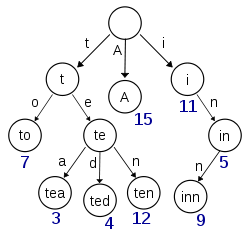
\includegraphics[width=.5\textwidth]{trie.png}
	\caption{A trie data type visualization}
\end{figure}



\subsection{Heap}

\rsrc{The Heap}\href{https://en.wikipedia.org/wiki/Heap_%28data_structure%29}{Wiki Link}

	Tree data type, subtype of a priority queue. two types \ra min and max. In a min/max heap the root is the lowest/highest value in the tree.

	The binary heap was introduced for the heap sort algorithm. The heap is partially ordered.

	\begin{itemize}
		\item Heap Property: with P \ra parent node, C \ra child node, then the key of P is ordered with respect to C. This applies for every child and parent.
		\item The root is the lowest or highest value
		\item Items always go in the next free slot. If it isnt in the right place compare to its parent and swap is the parent is smaller/larger.
	\end{itemize}


\subsection{Sets}
\rsrc{Sets}{\href{https://en.wikipedia.org/wiki/Set_(abstract_data_type)}{Wiki Link}

\subsubsection{Union}
	\subsubsection{Tagged Union}

\section{Hashes}

Hash function 

\subsection{Hash Table}

\rsrc{Hash Table}\href{https://en.wikipedia.org/wiki/Hash_table}{Wiki Link}

Hash tables tend to be faster than other table data structures, degrading to the same average lookup time of an unordered array only in the worst case senario.
If the hash function is complex and the entry count small, this advantage can be lost.


\begin{table}
\centering
	\caption{\textbf{Time Complexity}}
\begin{tabular}{lll}
	Algo&Ave&Worst\\
	Space&O(n)&O(n)\\
	Search&O(1)&O(n)\\
	Insert&O(1)&O(n)\\
	Delete&O(1)&O(n)\\
\end{tabular}
\end{table}
A hash table is an associative array (i.e. a dictionary) that maps keys to values. 
Puts a key through a hash function to find/retrieve an index to an array of buckets
\begin{table}
	\label{table:hashTableTerms}
	\caption{Hash table terms}
	\begin{tabular}{r p{.8\textwidth}}
		Key& The name of a value/ attribute\\
		Bucket& The array elements. Typically a dynamic array\\
		Slot& Synonym for bucket\\
		Hash function& computes the index from a key\\
		Load Factor& $\frac{entries}{buckets}$ The higher the load factorthe slower the search, the lower the load facter the more memory wasted.\\
	\end{tabular}
\end{table}

\subsubsection{Collision Resolution}
\begin{tabular}{r p{.8\textwidth}}
	Separate Chaining&Buckets have a list of their own entries to a single has, if the hash matches and the key doesn't do a linear search of the list\\
	Open Addressing&On a collision, the new entry takes the next open slot. Useful if memory is an issue and the entries are smaller that $\sim$ 4$\times$ sizeof(*)\\

\end{tabular}

